\chapter{Gestión de alcance}



\section{Objetivos del proyecto}
El objetivo del proyecto consta de la realización de una instalación ICT en un bloque de cinco plantas. La instalación estará formada por RTV, fibra óptica, televisión por cable y par trenzado. Entregaremos la instalación cuando se cumpla con todos los requisitos y obligaciones del Real Decreto 346/2011.

\section{Descripción del alcance del producto}
La instalación se realizará en un bloque de cinco pisos, constituido por un local en la planta inferior y cuatros plantas superiores. Esta instalación se llevará a cabo por dos instaladores de nuestra empresa. Éstos deberán instalar el cableado de canalización exterior, de enlace, principal, secundaria e interior del usuario. El diseño de las canalizaciones se hará a petición del cliente. A continuación se describirán los productos necesarios para cada instalación.
\begin{itemize}
\item \textbf{Instalación de RTV:} se necesitará cable coaxial, tomas RTV, amplificadores de señal, derivadores (por lo menos de tres tipos), repartidores y antenas(TV, FM y DAB); las antenas satélites quedan excluidas por petición del cliente.
\item \textbf{Instalación CATV:} se necesitará cable coaxial, un panel de distribución y tomas CATV.
\item \textbf{Instalación STDP:} se necesitará cable de par trenzado UTP de categoría 6 (por petición del cliente), un panel de distribución, roseta de terminación, multiplexores y tomas RJ-45.
\item \textbf{Instalación fibra óptica:} se necesitarán cable de fibra óptica sc/apc, panel de distribución y caja de conexiones.
\end{itemize}
Todas estas instalaciones se realizarán con los instrumentos necesarios y cumpliendo con la normativa y los requisitos del cliente.

\section{Requisitos del proyecto}
Tras mantener varias reuniones con el cliente, a continuación citaremos los requisitos pedidos:
\begin{itemize}
\item [$-$] Disponemos de 3 meses para realizar el proyecto.
\item [$-$] Debemos realizar la instalación completas de RTV, CATV y STDP.
\item [$-$] La instalación de fibra óptica se hará hasta cada PAU, por si en un futuro es necesario y solo se hará la instalación interior del usuario.
\item [$-$] NO  realizaremos la instalación de TVSat.
\item [$-$] Instalaremos el mínimo de tomas que debe haber en cada vivienda de un bloque de 5 PAUs. Este mínimo de tomas se especifica en la normativa.
\item [$-$] En la fecha de entrega, otorgaremos la instalación certificada por su buen funcionamiento y con dos manuales de usuario, uno en castellano y otro en catalán.
\item [$-$] El diseño de la canalización principal y secundaria se realizará, a petición del cliente, en el momento de la instalación.
\item [$-$] Los embellecedores de las tomas se escogerán por parte del cliente.
\item [$-$] La calidad de los materiales de la instalación (cables, distribuidores, etc.) serán de gama alta.
\end{itemize}
\section{Entregables}
Los entregables del proyecto serán los siguientes:
\begin{itemize}
\item La instalación ICT acabada.
\item El boletín del protocolo de pruebas.
\item Los manuales de usuario, uno en castellano y otro en catalán.
\item El documento de fin de obra.
\end{itemize}
\section{Criterios de Aceptación}
El proyecto será aceptado por el cliente si:
\begin{itemize}
\item [$-$] Todas las instalaciones a realizar están acabadas y funcionan correctamente.
\item[$-$] Todos los requisitos del cliente se cumplan. 
\end{itemize}
\section{Suposiciones del proyecto}
El edificio en el que realiza la ICT, damos por supuesto que es un edificio ordinario en el sentido de que no presente irregularidades que dificulten o supongan un problema para la instalación.
\section{Riesgos iniciales}
El riesgo inicial más importante que tenemos es que el presupuesto debe ser suficiente para realizar el proyecto. En caso de que el presupuesto no sea suficiente, nos vemos obligados a usar material de gama media e ignorar los embellecedores de toma o el diseño indicado a petición del cliente y, en su lugar, proporcionar unos de menor presupuesto que se puedan permitir para que la instalación pueda finalizar correctamente. \\
Otro riesgo inicial es que fallemos en los cálculos preliminares y, a causa de esto, tengamos niveles de toma con una relación señal/ruido regular. Para evitar esto, iremos realizando cálculos preliminares de forma periódica mientras se ejecuta la instalación. También corremos el riesgo de que el cliente cambie o añada requisitos.
\section{Estructura Desglosada del Trabajo del proyecto (EDT)}
A continuación se muestra la EDT por fases del proyecto:
\begin{figure}[H]
\centering
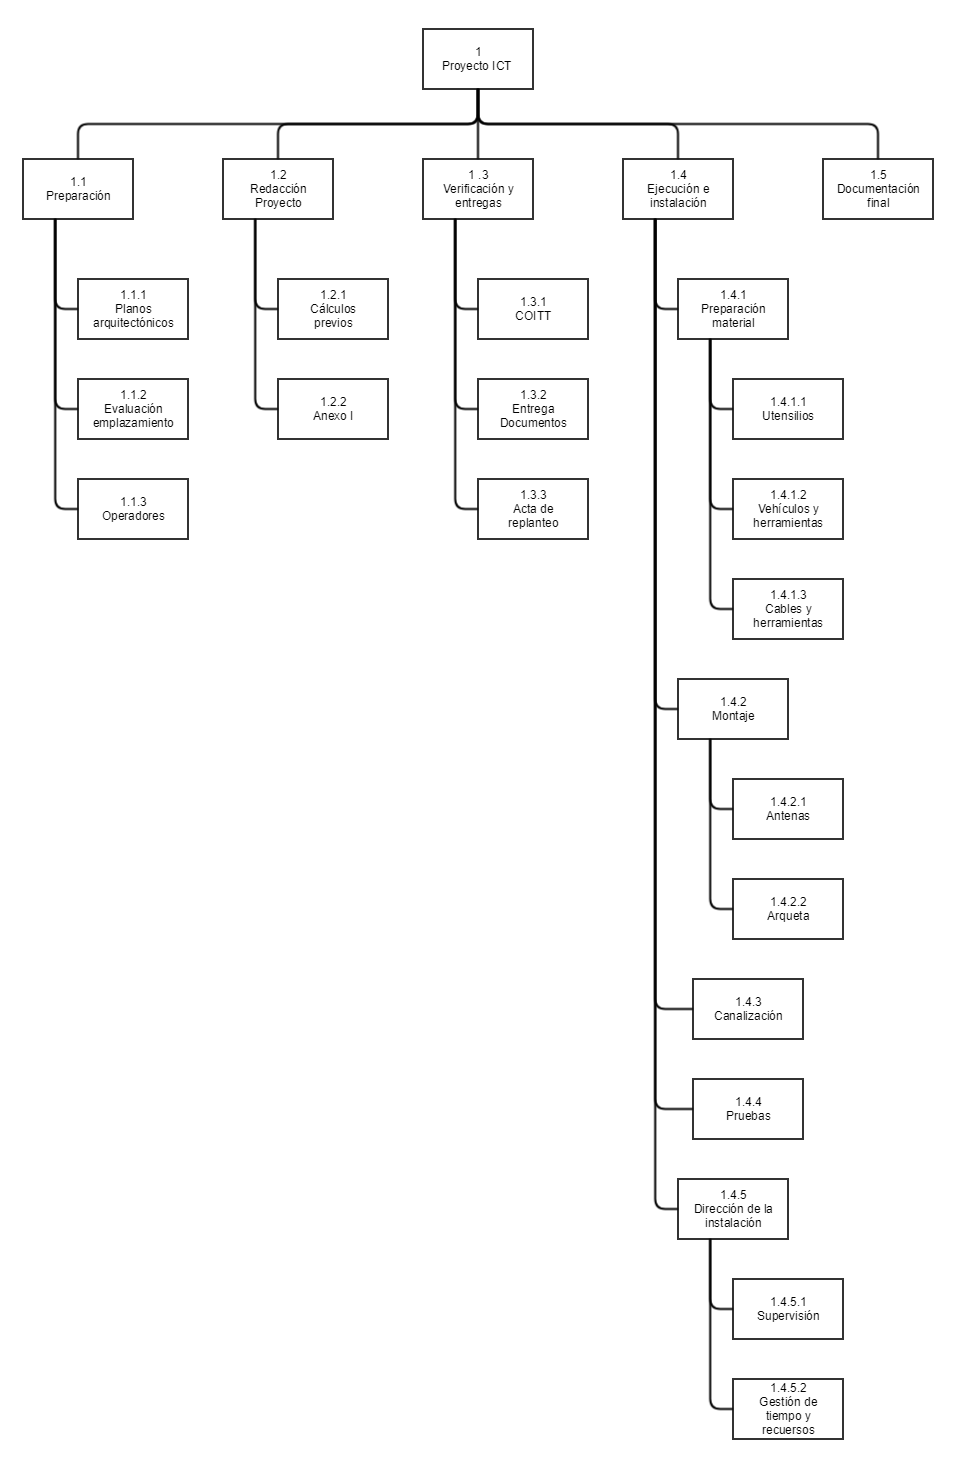
\includegraphics[scale = 0.55]{project/images/edt.png}
\caption{Estructura EDT}
\end{figure}
%%%%%%%%%%%%%%%%%%%%%%%%%%%%%%%%%%%%%%%%%%%%%%%%%%%%%%%%%%%%%%
%Aquí esta el diccionario, sobre la posición me daba errores no lo se porque bueno, una vez acabado se verá sobre la posición por ahora rellenar esto y luego haremos cambios, es fácil entender esta tabla así que no creo que tengan problemas.
%\newgeometry{left = 1.5cm,right = 1cm}
\begin{table}[H]
\begin{tabular}{|m{1cm}|m{2cm}|m{5cm}|m{2cm}|m{2.5cm}|m{2.8cm}| }
\hline
 \multicolumn{6}{|c|}{\centering Diccionario} \\
\hline
\rowcolor{gray!50}  \centering EDT código & \centering Código (EDT) & Actividades y Definición & Responsables & Fecha & Dependencias \\
\hline
  \centering 1\\ (nv 1) & \centering Proyecto ICT & Se realizará una proyecto para implementar una ICT. & \centering Director &Inicio: 18/12/17 Fin: 18/03/18& Ninguna \\
\hline
  \centering 1.1\\ (nv 2) & \centering Preparación & Preparar los documentos y mantener comunicaciones previas  a  la redacción del proyecto \. & \centering Director y Jefe de proyecto &Inicio: 18/12/17 Fin: 23/12/17 & Antes de (1.2) \\
\hline
 \centering 1.1.1\\ (nv 3) & \centering Planos arquitectónicos & (A) Comunicarse con el Arquitecto para facilitar los planos en fase de final de la obra. & \centering  Director &Inicio: 18/12/17 Fin: 18/12/17 & Antes de (1.1.2)\\
\hline
 \centering 1.1.2\\ (nv 3) & \centering Evaluación emplazamiento &  Observación de la ubicación: (A) Observar edificios del alrededor para cálculo de sombra radioeléctrica; (B) Observar si hay existencia de dotación de servicios; (C) Evaluar el estado de las redes de telecomunicación de la zona; (D) Obtener medidas de potencia de señal. & \centering Ingenieros e Instaladores &Inicio: 19/12/17 Fin: 19/12/17 & Después de (1.1.1) \\
\hline
 \centering 1.1.3\\ (nv 3) & \centering Operadores & (A) Consultar de forma telemática con los operadores para definir qué redes no se van a implementar.& \centering Jefe de proyecto &Inicio: 19/12/17 Fin: 20/12/17 & Ninguna\\
\hline
\centering 1.2\\ (nv 2) & \centering Redacción proyecto & Fase de redacción del proyecto de ICT. & \centering Jefe de proyecto &Inicio: 25/12/17 Fin: 07/01/18& Después de (1.1) Antes de (1.3)\\
\hline
 \centering 1.2.1\\ (nv 3) & \centering Cálculos previos & (A) Elección del tipo de cableado, (B) Realizar propósito de distribución similar de los niveles de atenuación y de señal, esquema de red, elementos y dimensión de RTV, planos de infraestructura y (C) Colocar de la arqueta de entrada sobre el plano. & \centering Ingenieros &Inicio: 25/12/17 Fin:30/12/17& Después de 1.1.2\\
\hline
 \centering 1.2.2\\ (nv 3) & \centering Anexo I & (A) Rellenar según el Anexo I. & \centering Jefe de Proyecto &Inicio: 26/12/17 Fin: 07/01/18& Ninguna\\
\hline
 \centering 1.3\\ (nv 2) & \centering Verificación y entregas & Trámites de verificación y entregas que se deben realizar del proyecto. & \centering Director &Inicio: 09/01/18 Fin: 10/01/18& Después de (1.2) Antes de (1.4) \\
\hline
 
\end{tabular}
%Lo que sigue lo pueden quitar si lo desean, no sabía si al final habra que hacer como un lugar especial donde irán todas las tablas

\caption{Diccionario del EDT}
\label{table:ta}
\end{table}
\begin{table}[H]
\begin{tabular}{|m{1cm}|m{2cm}|m{5cm}|m{2cm}|m{2.5cm}|m{2.8cm}| }
\hline
 \multicolumn{6}{|c|}{\centering Diccionario} \\
\hline
\rowcolor{gray!50} \centering EDT código & \centering Código (EDT) & Actividades y Definición & Responsables & Fecha & Dependencias \\
\hline
\centering 1.3.1\\ (nv 3) & \centering COITT & (A) Entregar el proyecto al Colegio Oficial de Ingenieros Técnicos de Telecomunicación. (B) Recibir verificación. & \centering Director &Inicio: 09/01/18 Fin: 09/01/18 & Ninguna\\
\hline
 \centering 1.3.2\\ (nv 3) & \centering Entrega documentos & (A) Entregar una copia del proyecto a la Propiedad. (B) Entregar una copia del proyecto al Ministerio. & \centering Director & Inicio: 10/01/18 Fin: 10/01/18& Ninguna\\
\hline
\centering 1.4\\ (nv 2) & \centering Ejecución e instalación & Procesos de ejecución e instalación en la infraestructura en la que se realiza el proyecto ICT. & Director e Ingenieros & Inicio: 23/01/18 Fin: 10/03/18& Después de (1.3) \\
\hline
 \centering 1.4.1\\ (nv 3) & \centering Preparación material & Preparación el material que se utilizará para la instalación del proyecto.& Instaladores & Inicio: 23/01/18
 Fin: 24/01/18& Antes de (1.4.2)\\
\hline
 \centering 1.4.1.1\\ (nv 4) & \centering Utensilios & (A) Preparación de los utensilios. (B) Presentación de los utensilios en el edificio. & Instaladores & Inicio: 23/01/18 Fin:23/01/18& Ninguna \\
\hline
 \centering 1.4.1.2\\ (nv 4) & \centering Vehículos y herramientas & (A) Preparación de vehículos y herramientas. (B) Presentación de vehículos y herramientas en el edificio. & Instaladores & Inicio: 23/01/18 Fin:24/01/18& Ninguna \\
\hline
 \centering 1.4.1.3\\ (nv 4) & \centering Cables y canalización & (A) Preparación del cableado. (B) Presentación del cableado en el edificio. & Instaladores & Inicio: 24/01/18 Fin: 24/01/18 & Ninguna \\
\hline
 \centering 1.4.2\\ (nv 3) & \centering Montaje & Fase de montaje de las infraestructuras del proyecto.& Instaladores & Inicio: 25/01/18 Fin: 18/02/18& Después de (1.4.1) Antes de (1.4.3) \\
\hline
 \centering 1.4.2.1\\ (nv 4) & \centering Antenas &
(A) Montaje de antenas. & Instaladores & Inicio: 25/01/18 Fin: 18/02/18& Ninguna \\
 \hline
 \centering 1.4.2.2\\ (nv 4) & \centering Arqueta &
 (A) Montaje de la arqueta de entrada. (B) Conectividad de la arqueta de entrada. & Instaladores & Inicio: 25/01/18 Fin: 18/02/18 & Ninguna \\
\hline
 \centering 1.4.3\\ (nv 3) & \centering Canalización & 
(A) Instalación del cableado. (B) Montaje de los embellecedores. & Instaladores & Inicio: 19/02/18 Fin: 03/03/18 & Después de (1.4.2) Antes de (1.4.4) Antes de (1.5) \\
\hline
 \centering 1.4.4\\ (nv 3) & \centering Pruebas & 
 (A) Realización de pruebas del funcionamineto de la instalación. & Ingenieros & Inicio: 05/03/18 Fin: 10/03/18 & Después de (1.4.3)\\
\hline
 
\end{tabular}
%Lo que sigue lo pueden quitar si lo desean, no sabía si al final habra que hacer como un lugar especial donde irán todas las tablas
\caption{Diccionario del EDT}
\label{table:ta1}
\end{table}
\begin{table}[H]
\begin{tabular}{|m{1cm}|m{2cm}|m{5cm}|m{2cm}|m{2.5cm}|m{2.8cm}| }
\hline
 \multicolumn{6}{|c|}{\centering Diccionario} \\
\hline
\rowcolor{gray!50} \centering EDT código & \centering Código (EDT) & Actividades y Definición & Responsables & Fecha & Dependencias \\
\hline
 \centering 1.4.5\\ (nv 3) & \centering Dirección de la Instalación & El proceso de instalación se debe supervisar para que transcurra según lo planeado. También hay que gestionar los imprevistos en la administración del tiempo y las posibles faltas de recursos.& \centering Director & Inicio: 23/01/18 Fin: 10/03/18 & Durante (1.4) \\
\hline
 \centering 1.4.5.1\\ (nv 4) & \centering Supervisión & 
(A) Comprobación de proceso de instalación. (B) Resolución de dudas. (C) Resolución de conflictos. & \centering Director e Ingenieros& Inicio: 23/01/18 Fin: 10/03/18 & Ninguna \\
 \hline
 \centering 1.4.5.2\\ (nv 4) & \centering Gestión de tiempo y recursos & (A) Reajustes de planificación temporal. (B) Reajustes de presupuesto. & \centering Director y Jefe de proyecto & Inicio: 23/01/18 Fin: 10/03/18 & Ninguna \\
\hline
 \centering 1.5\\ (nv 2) & \centering Documentos finales & (A) Realizar boletín de instalación.
(B) Realización de protocolos de prueba.
(C) Realización de manual de usuario. & \centering Director & Inicio: 12/03/18 Fin: 18/03/18 & Después de (1.4.3) \\
\hline
\end{tabular}
\caption{Diccionario del EDT}
\label{table:ta1}
\end{table}

%%%%%%%%
\subsection{Hitos}

\begin{itemize}

\item Inicio del proyecto - Inicio de (1).
\item Completar la redacción del proyecto - Fin de (1.2).
\item Verificación del proyecto - Fin de (1.3.1).
\item Inicio de la instalación - Inicio de (1.4).
\item Terminar el proceso de montaje e instalación - Fin de (1.4.3).
\item Finalización del proyecto - Fin de (1).

\end{itemize}
%%%%%%%
\newpage
